\documentclass{beamer}
%\documentclass[handout,t]{beamer}

\batchmode
% \usepackage{pgfpages}
\usepackage{tikz}
% \usetikzlibrary{patterns}
% \usetikzlibrary{matrix}
% \usetikzlibrary{graphs}
% \usetikzlibrary {chains,scopes}
% \usetikzlibrary {arrows.meta,automata,positioning}
% \pgfpagesuselayout{4 on 1}[letterpaper,landscape,border shrink=5mm]

\usepackage{amsmath,amssymb,enumerate,epsfig,bbm,calc,color,ifthen,capt-of}
\usepackage{macros}

\usetheme{Berlin}
\usecolortheme{mit}

\title{Feedback Linearizable Discretizations of Mechanical Systems using Retraction Maps} 
\subtitle{BTP Stage I Presentation}
\author[Shreyas N B]{Shreyas N B \\ [1.5ex] {\small Guide: Prof. Ravi Banavar} \\ {\small Co-Guide: Prof. Krishnendu Haldar}} 
\institute[IIT Bombay]{B. Tech, Department of Aerospace Engineering\\ IDDDP, Center for Systems and Control }
\date{\today}

\logo{
\includegraphics[height=1cm]{../Figures/iitblogo.png}}

\AtBeginSection[]
{
  \begin{frame}<beamer>
    \frametitle{Outline}
    \tableofcontents[currentsection]
  \end{frame}
}
\beamerdefaultoverlayspecification{<+->}
% -----------------------------------------------------------------------------
\begin{document}
% -----------------------------------------------------------------------------

\frame{\titlepage}

\section[Outline]{}
\begin{frame}{Outline}
  \tableofcontents
\end{frame}

% -----------------------------------------------------------------------------
\section{Introduction}



\subsection{Feedback Linearization}

\begin{frame}{Motivation}
  Consider a continous-time nonlinear system of the form:

  \[ \dot{x}(t) = f(x(t), u(t)) \]
  
  Assuming the following:
  \begin{enumerate}
    \item There exists a coordinate transformation $z := \varphi(x)$ and an auxiliary control $v : = \psi(x,u)$ such that $\dot{z}(t) = Az(t) + Bv(t)$ where $A, B$ are constant matrices.
    \item The discretization scheme is arbitrary.
  \end{enumerate}

\end{frame}

\begin{frame}{Motivating Example}
  \begin{equation}
    \pmat{\dot{x}_1 \\ \dot{x}_2} = \pmat{(1+2u(t))x_2(t) \\ u(t)}
\end{equation}

Taking $\tilde{x}_1 = x_1 - x_2^2$ and $\tilde{x}_2 = x_2$, we get the transformation $\varphi(x_1, x_2) = \left(x_1 - x_2^2, x_2 \right)$, we get the feedback linearized system:

\begin{equation}
\pmat{\dot{z}_1(t) \\ \dot{z}_2(t)} = \pmat{z_2(t) \\ u(t)}
\end{equation}
\end{frame}

\begin{frame}{Definitions}
\begin{block}{Continuous Feedback Linearization}
  A continous-time nonlinear system $\dot{x}(t) = f(x(t), u(t))$ is said to be feedback linearizable if there exists a coordinate transformation $z = \varphi(x)$ and a feedback control law $v = \psi(x,u)$ such that the transformed system is linear $\dot{z}(t) = Az(t) + Bv(t)$.
\end{block}

\begin{block}{Discrete Feedback Linearization}
  A discrete-time nonlinear system $x_{k+1} = F(x_k, u_k)$ is said to be feedback linearizable if there exists a coordinate transformation $z_k = \varphi(x_k)$ and a feedback control law $v_k = \psi(x_k,u_k)$ such that the transformed system is linear $ z_{k+1} = Az_k + Bv_k $, where $x_k = x(t_k)$.
\end{block}

\end{frame}

\begin{frame}{Motivating Example}
  \begin{equation}
    \pmat{\dot{x}_1 \\ \dot{x}_2} = \pmat{(1+2u(t))x_2(t) \\ u(t)}
\end{equation}

Taking $\tilde{x}_1 = x_1 - x_2^2$ and $\tilde{x}_2 = x_2$, we get the diffeomorphism $\varphi(x_1, x_2) = \left(x_1 - x_2^2, x_2 \right)$, we get the feedback linearized system:

\begin{equation}
\pmat{\dot{z}_1(t) \\ \dot{z}_2(t)} = \pmat{z_2(t) \\ u(t)}
\end{equation}
\end{frame}

\begin{frame}{Type 1 Discretization}

First, we consider the forward Euler discretization scheme. This gives a discrete-time system:

\begin{equation}
\pmat{x_{1,k+1} \\ x_{2, k+1}} = \pmat{x_{1,k} \\ x_{2,k}} + h\pmat{(1+2u_k)x_{2,k} \\ u_k}
\end{equation}

Taking the same diffeomorphism $\varphi$ as before, we get:

\begin{equation}
\pmat{z_{1,k+1} \\ z_{2,k+1}} = \pmat{z_{1,k} + hz_{2,k} - h^2 u_k^2 \\ z_{2,k} + h u_k}
\end{equation}

Thus, we see that it is NOT feedback linearizable.

\end{frame}

\begin{frame}{Type 2 Discretization}
Now, let's consider an alternate discretization which yields the discrete system:

\begin{equation}
\pmat{x_{1,k+1} \\ x_{2, k+1}} = \pmat{x_{1,k} \\ x_{2,k}} + h\pmat{(1+2u_k)x_{2,k} \\ u_k} + h^2 \pmat{u_k^2 \\ 0}
\end{equation}

Again taking the same diffeomorphism $\varphi$, we get:

\begin{equation}
\pmat{z_{1,k+1} \\ z_{2,k+1}} = \pmat{z_{1,k} + hz_{2,k} \\ z_{2,k} + h u_k}
\end{equation}

which is indeed feedback linearizable.

\end{frame}

\begin{frame}{Motivation}

  \begin{block}{Question 1}
    Can we construct a discretization scheme such that the discrete system can also be linearized using $\varphi(x)$ and $\psi(x,u)$ similarly?
  \end{block}
  
  \begin{block}{Question 2}
    Can we extend this scheme (geometrically) to second-order nonlinear mechanical systems?
  \end{block}
  
\end{frame}

\begin{frame}{Motivation}
  \begin{figure}[h]
    \centering
    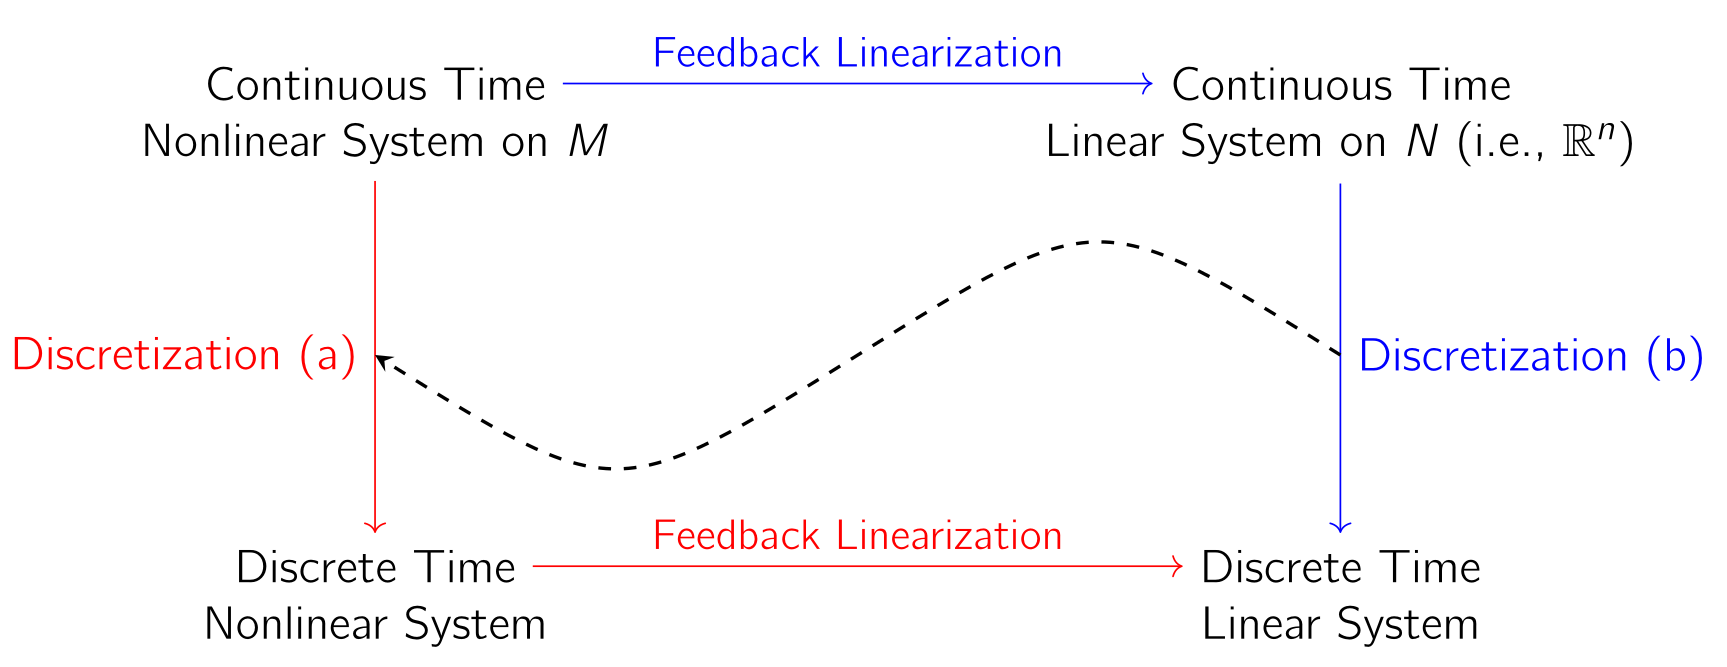
\includegraphics[width=\textwidth]{../Figures/feedback_lin.png}
    \caption{\textsl{Feedback Linearizable} Discretization?}
  \end{figure}
  
\end{frame}

\begin{frame}{Observations}
  \begin{block}{Problem}
    Feedback linearizability of discrete-time systems depends on the choice of the discretization scheme.
  \end{block}

  \begin{block}{Objective}
    Given a (locally) feedback linearizable continuous-time nonlinear system, construct a discretization scheme such that the discrete-time system is also (locally) feedback linearizable.
  \end{block}

  \begin{block}{Strategy}
    We utilize the concept of \textbf{retraction maps} to construct such a discretization scheme.
  \end{block}
  
\end{frame}
% 

\subsection{Retraction and Discretization Maps}

\begin{frame}{Definition}
  We define a \textbf{retraction map} on a manifold $M$ as a smooth map $\Ret: TM \to M$, such that if $\Ret_x$ be the restriction of $\Ret$ to $T_x M$, then the following properties are satisfied:

    \begin{enumerate}
        \item $\Ret_x (0_x) = x$ where $0_x$ is the zero element of $T_x M$.
        \item $\text{D}\Ret_x (0_x ) = T_{0_x} \Ret_x = \mathbb{I}_{T_x M} $, where $\mathbb{I}_{T_x M}$ is the identity mapping on $T_x M$.
    \end{enumerate}
  
\end{frame}

\begin{frame}{Retraction Map}
\begin{figure}
  \centering
  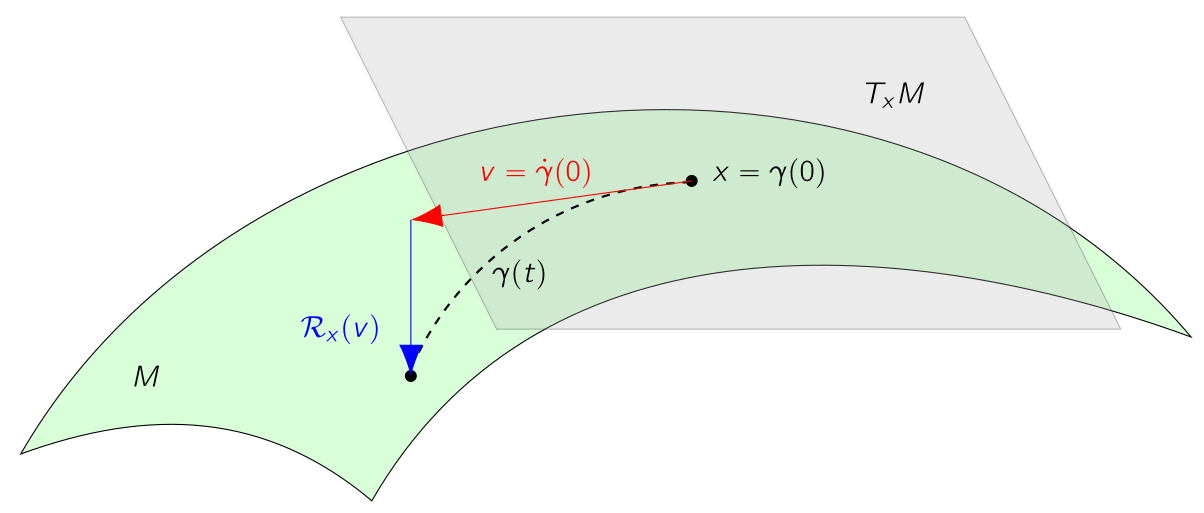
\includegraphics[width=\textwidth]{../Figures/retraction.png}
  \caption{A visualization}
\end{figure}
\end{frame}

\begin{frame}{Discretization Map}
  A map $\D : U \subset TM \longrightarrow M \times M$ given by 

\[
  \D (x,v) \equiv \D_x(v) = \left( R^1_x(v), R^2_x(v) \right)
\]

where $U$ is the open neighborhood of the zero section $0_x \in TM$, is called a \textbf{discretization map} on $M$, if the following properties are satisfied:

\begin{enumerate}
  \item $\D(x,0_x) = (x,x)$ 
  \item $T_{0_x}R_x^2 - T_{0_x}R_x^1 = \mathbb{I}_{T_x M}$, which is the identity map on $T_x M$ for any $x \in M$.
\end{enumerate}
  
\end{frame}

\begin{frame}{Discretization Map}
  Some examples of discretization maps on $\R[n]$ for $\dot{x}(t) = X(x(t))$:

  \begin{figure}
    \centering
    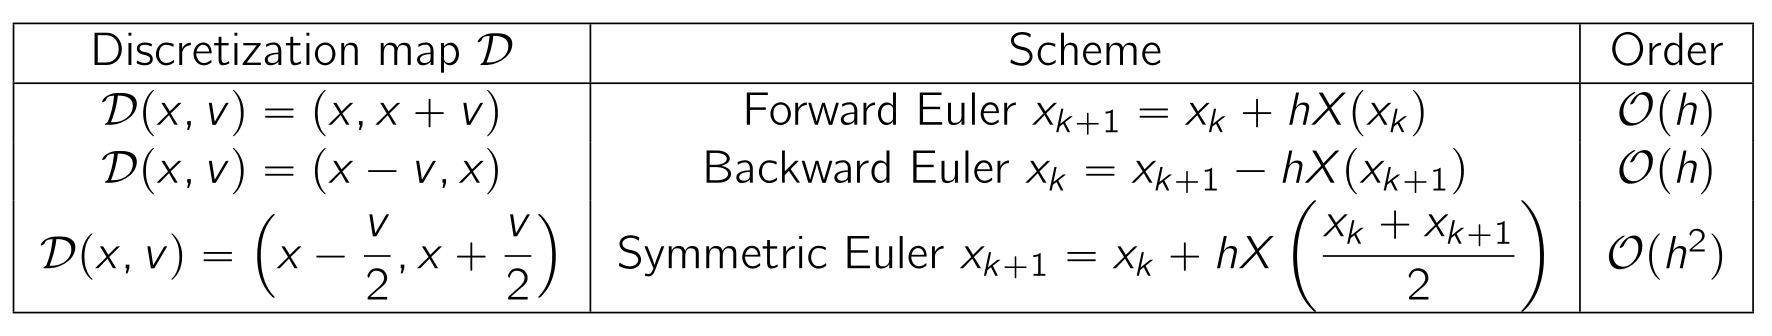
\includegraphics[width=\textwidth]{../Figures/discretizations.png}
  \end{figure}
\end{frame}

\section{Feedback Linearizable Discretizations}

\begin{frame}{Notations}

  \begin{itemize}
    \item $\mathfrak{X}(M)$ : set of all vector fields on $M$. 
    \item $\dot{x}(t) = X(x(t))$ : dynamical system defined by $X \in \mathfrak{X}(M)$.
    \item $\tau_M : TM \longrightarrow M$ : canonical projection $M$ s.t. $\tau_M(x,v) = x$.
    \item $h = t_{k+1} - t_k$ : time step of discretization.
    \item $\D^{TM}$ is a discretization map on $M$.
  \end{itemize}
  
\end{frame}

\subsection{Discretization of Vector Fields}
\begin{frame}{Discretization of Vector Fields}
  \begin{block}{Proposition}
    Let $X(\cdot, u_k) \in \mathfrak{X}(M)$ be a controlled vector field on $M$. Then, for a given discretization scheme $\D$,

    \[
      \D^{-1}(x_k, x_{k+1}) = hX(\tau_M(\D^{-1}(x_k, x_{k+1})), u_k)
    \]

    is an implicit numerical discretization of $\dot{x}(t) = X(x(t), u(t))$.
  \end{block}


  \begin{block}{Example}

    The forward Euler discretization scheme $\D(x,v) = (x, x + v)$ yields the explicit Euler form $x_{k+1} = x_k + hX(x_k, u_k)$.
    
  \end{block}
  
\end{frame}

\subsection{Lift of Discretization Maps}
\begin{frame}{Tangent Lift}
  \begin{block}{Proposition}
    Let $\varphi: M \lra N$ be a smooth map (diffeomorphism). For a given discretization map $\D^{TM} : TM \lra M \times M$ on $M$, the map $\D^{TN} :=  (\varphi \times \varphi) \circ \D^{TM} \circ T \varphi ^{-1}$ is a discretization map on $N$ i.e., $\D^{TN} : TN \lra N \times N$.
  \end{block}

  \begin{figure}[h]
    \centering
    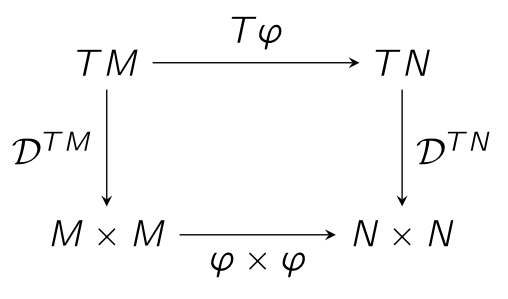
\includegraphics[width=0.5\textwidth]{../Figures/commutator.png}
  \end{figure}
\end{frame}

\begin{frame}{Feedback Linearizable Discretization}
  \begin{block}{Proposition}
    Let $\varphi$ be the linearizing coordinate transformation and $\psi$ be the linearizing feedback. Let $\D^{TN}$ be a discretization map that \textbf{discretizes the continuous-time linear system to a discrete-time linear system}. Then,

    \[
      \D^{TM} = (\varphi \times \varphi)^{-1} \circ \D^{TN} \circ T \varphi
    \]

    is a discretization on $M$ which discretizes the continuous-time system to a discrete-time nonlinear system such that the discrete-time system is feedback linearizable using $z_k : = \varphi(x_k)$ and $v_k : = \psi(x_k, u_k)$.
  \end{block}
  
\end{frame}

\section{Second-Order Systems}

\subsection{Second-Order Differential Equations}

\begin{frame}{Motivation}
  \begin{enumerate}
    \item Mechanical systems are usually described by nonlinear second-order differential equations (SODEs).
    \item These systems also have underlying mechanical structures (symmetry, conservation laws, etc.) which needs to be preserved while linearizing and discretizing.
    \item Since the notion of mechanical feedback linearization has been well-studied, it is natural to extend this to the discrete-time setting.
  \end{enumerate}
\end{frame}

\begin{frame}{Second Order Differential Equations}
  A second-order differential equation (SODE) is a vector field $X$ such that locally,
  \begin{equation}
      X = \dot{x}^i \frac{\partial}{\partial x^i} + X^i(x^i, \dot{x}^i) \frac{\partial}{\partial \dot{x}^i}
  \end{equation}
  To find the integral curves of $X$ is equivalent to solving the SODE:
  \begin{equation}
  \label{eq:sode}
      \frac{d^2}{dt^2}x(t) = X \left( x(t), \frac{d}{dt}x(t) \right) 
  \end{equation}

\end{frame}

\begin{frame}{Discretization of SODEs}
  Now, we wish to discretize this using the notion of the discretization map on $TM$. We would like to tangently lift a discretization on $M$ to obtain $\D^{TTM}: TTM \lra TM \times TM$. This yields the following numerical scheme:
  \begin{equation}
  \label{eq:disc}
  \begin{split}
    {\left(\D^{TTM}\right)}^{-1} & (x_k, y_k; x_{k+1}, y_{k+1}) \\ = h X & \left( \tau_{TM} \left( {\left(\D^{TTM}\right)}^{-1}(x_k, y_k; x_{k+1}, y_{k+1})\right)\right)
  \end{split}
  \end{equation}
  
\end{frame}

\begin{frame}{What is different here?}

  The double tangent bundle $TTM$ admits two different vector bundle structures:

  \begin{enumerate}
    \item The canonical vector bundle with projection $\tau_{TM} : TTM \lra TM$.
    \item The vector bundle given by the projection of the tangent map $T \tau_M : TTM \lra TM$. 
  \end{enumerate}

  \pause
  Denote the canonical involution map $\kappa_M : TTM \lra TTM$ which is a vector bundle isomorphism, over the identity of $TM$.

\[
 \kappa_M (x, v, \dot{x}, \dot{v}) = (x,\dot{x}, v, \dot{v})
\]
  
\end{frame}

\begin{frame}{Why is this important?}
  The tangent lift of a vector field $X$ on $M$ does not define a vector field on $TM$. It is necessary to consider the composition $\kappa_M \circ TX$ to obtain a vector field on $TM$, and this is called the \textbf{complete lift} $X^c$ of the vector field $X$. 
  Hence, a similar technique must be used to lift a discretization map from $TM$ to $TTM$.

  \begin{block}{Proposition}
    If $\D^{TM} : TM \lra M \times M$ is a discretization map on $M$, then $\D^{TTM} = T\D^{TM} \circ \kappa_M$ is a discretization map on $TM$.
  \end{block}
  
\end{frame}

\begin{frame}{Tangent Lift of Discretization Map}
  \begin{figure}[h]
    \centering
    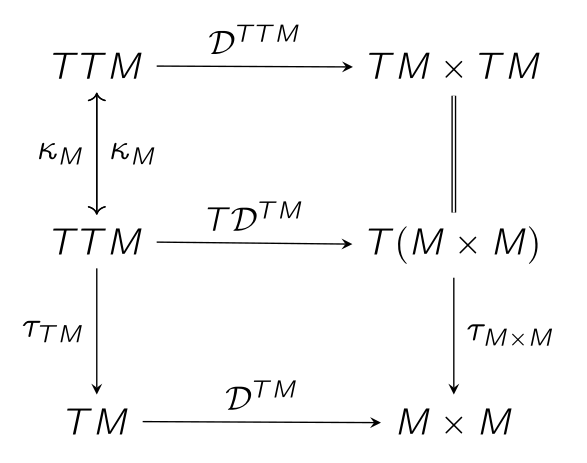
\includegraphics[width=0.5\textwidth]{../Figures/double-tangent.png}
    \caption{Commutation of maps around $TTM$}
  \end{figure}
  
\end{frame}

\begin{frame}{The whole (slightly intimidating) picture}
  \begin{figure}
    \centering
    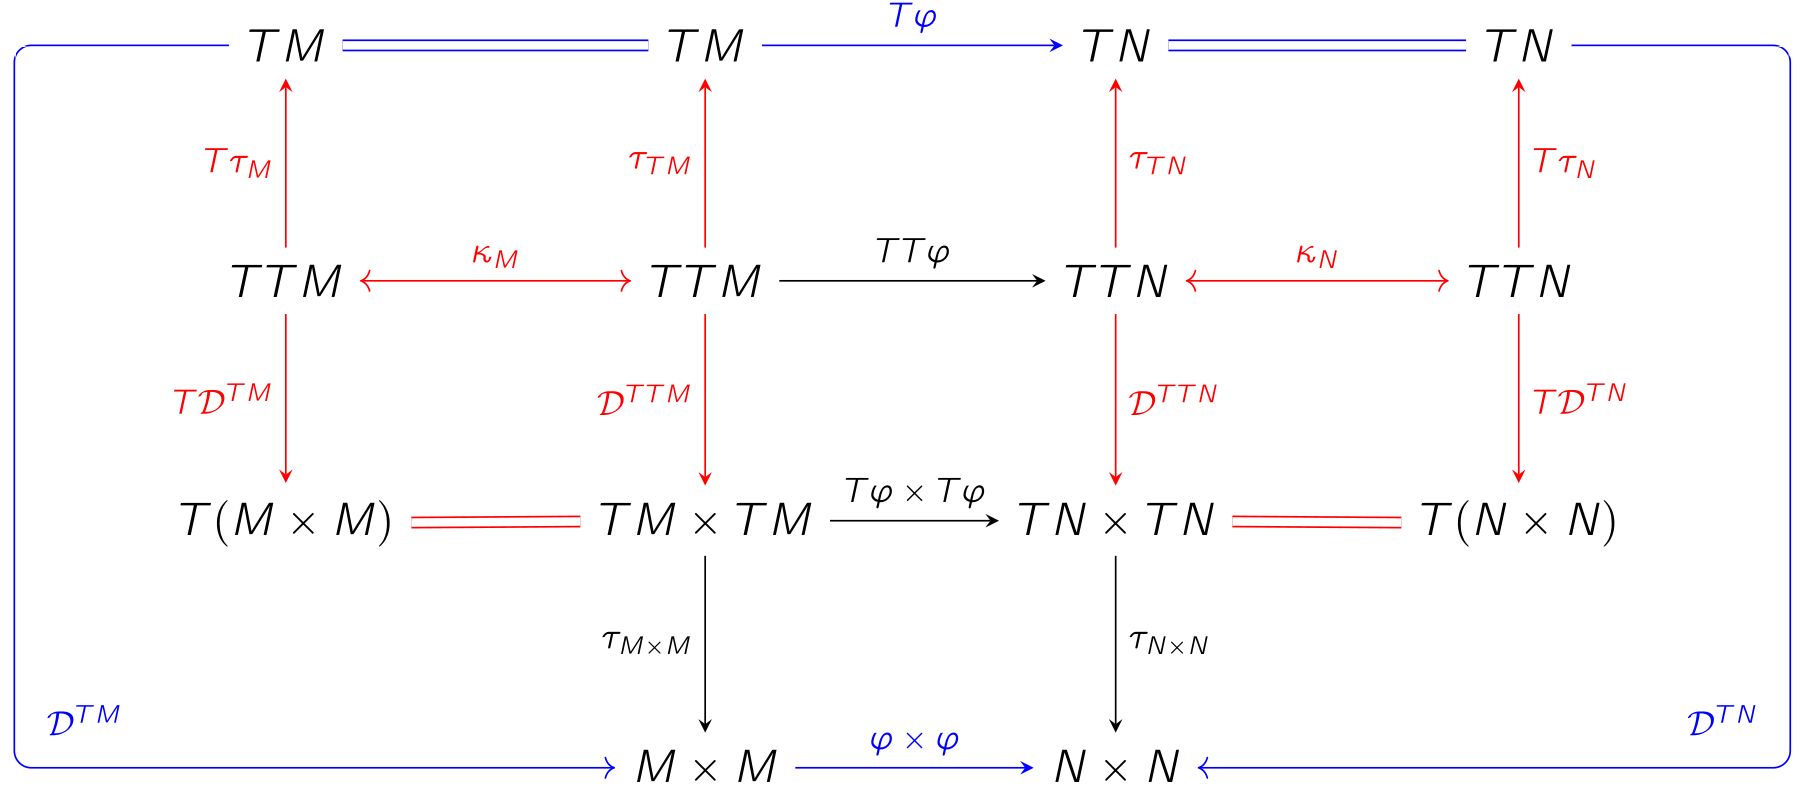
\includegraphics[width=\textwidth]{../Figures/double-commutator.png}
    \caption{The Commutator}
  \end{figure}
\end{frame}

\subsection{Mechanical Systems}

\begin{frame}{More Notation}

  \begin{itemize}
    \item $\Gamma^i_{jk}$ : Christoffel symbols (connection coefficients) on $M$.
    \item $\nabla$ : symmetric affine connection on $M$.
    \item $x = (x^1, \dots, x^i, \dots x^n)$ : local coordinates on $M$.
    \item $\mathfrak{g} = \{g_1,  \dots, g^r, \dots, g_m\}$ : control vector fields.
    \item $e$ : uncontrolled vector field.
  \end{itemize}
  
\end{frame}

\begin{frame}{Definition}
  \begin{block}{Mechanical Systems}
    A mechanical control system $(\mathcal{MS})_{(n,m)}$ is defined by a $4$-tuple $(M, \nabla, \mathfrak{g}, e)$ where:
    \begin{equation}
      \label{eq:mech}
      m\nabla_{\dot{x}} \dot{x} = e(x) + \sum_{r=1}^m g_r(x) u_r 
  \end{equation}
  Or equivalently in local coordinates $x = (x^1, \dots, x^n)$ on $M$, 
  \begin{equation}\label{SODE-initial}
      m\ddot{x}^i = - \Gamma ^i_{jk}(x)\dot{x}^j \dot{x}^k + e^i(x) + \sum_{r=1}^m g^i_r(x)u_r
  \end{equation}
    
  \end{block}
\end{frame}

\begin{frame}{Definition}
  We can write this as two first-order differential equations:
  \begin{equation}\label{SODE-nonlinear}
      \begin{split}
          \dot{x}^i  &= y^i; \\
          \dot{y}^i  &= - \Gamma^i_{jk}(x)y^jy^k + e^i(x) + \sum_{r=1}^m g_r^i(x)u_r
      \end{split} \tag{$\mathcal{MS}$} 
  \end{equation}

  \begin{block}{Conclusion}
    Given a mechanical control system $(\mathcal{MS})_{(n,m)}$, we wish to construct a discretization scheme such that the discrete-time system is \textbf{mechanical feedback linearizable}.
  \end{block}
  
\end{frame}

% \begin{frame}{Mechanical Feedback Linearizability}
%   \begin{equation*}
%         \mathcal{E}^0 = \text{span} \{ g_r, 1 \leq r \leq m \} \ ; \ \mathcal{E}^j = \text{span} \{ \text{ad}^i_e g_r, 1 \leq r \leq m, 0 \leq i \leq j \}
% \end{equation*}

% \begin{thm}\label{thm:mfl}
%     A mechanical system $(\mathcal{MS})_{(n,m)}$ is mechanical feedback ($MF$) linearizable, locally around $x_0 \in M$ iff, in the neighborhood of $x_0$:

%     \begin{itemize}
%         \item $(ML1)$ $\mathcal{E}^0$ and $\mathcal{E}^1$ are of constant rank
%         \item $(ML2)$ $\mathcal{E}^0$ is involutive
%         \item $(ML3)$ $\text{ann } \mathcal{E}^{0} \subset \text{ann } \mathfrak{R}$
%         \item $(ML4)$ $\text{ann } \mathcal{E}^0 \subset \text{ann } \nabla g_r \ \forall r: 1 \leq r \leq m$
%         \item $(ML5)$ $\text{ann } \mathcal{E}^1 \subset \text{ann } \nabla^2 e$
%     \end{itemize}

% \end{thm}
% \end{frame}

% \begin{frame}{Mechanical Feedback Linearizability}

% For planar mechanical systems ($n=2$):

% \begin{prop}
% \label{prop:planar_mech}
% A planar mechanical system $\mathcal{(MS)}_{(2,1)}$ is locally $MF$-linearizable at $x_0 \in M$ to a controllable $\mathcal{(LMS)}_{(2,1)}$, if and only if it satisfies the following conditions:
% \begin{enumerate}
%     \item $(MD1)$ $g$ and $\text{ ad}_e g$ are independent
%     \item $(MD2)$ $\nabla_g g \in \mathcal{E}^0$ and $\nabla_{\text{ad}_e g} g \in \mathcal{E}^0$
%     \item $(MD3)$ $\nabla^2_{g, \text{ad}_e g} \text{ad}_e g - \nabla^2_{\text{ad}_e g, g} \text{ad}_e g \in \mathcal{E}^0$
% \end{enumerate}
% \end{prop}
% \end{frame}

\section{Results}

\subsection{Inertia Wheel Pendulum}

\begin{frame}{Inertia Wheel Pendulum}
  \begin{figure}
    \centering
    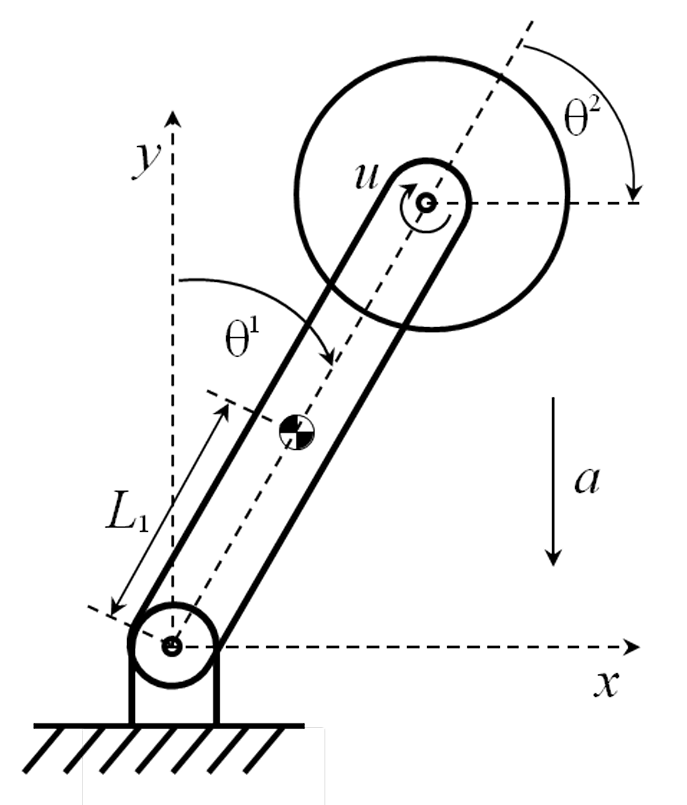
\includegraphics[width=0.4\textwidth]{../Figures/inertia_wheel.png}
    \caption{Mechanism}
  \end{figure}
\end{frame}

\begin{frame}{Inertia Wheel Pendulum - The Dynamical Equations}
  The equations of motion ($M = S^1 \times S^1$) are given by:
  \begin{equation}
    \begin{split}
        (m_d + J_2) & \Ddot{\theta}^1 + J \Ddot{\theta}^2 - m_0 \sin{\theta^1} = 0\\ 
        & J \Ddot{\theta}^1 + J \Ddot{\theta}^2 = u
    \end{split}
\end{equation}

where 
\begin{equation*}
    \begin{split}
        m_d  = L_1^2(m_1 + 4 m_2) + J_1, \
        m_0  = a L_1(m_1 + 2m_2)
    \end{split}
\end{equation*}
$m_1$ - mass of the pendulum, $m_2$ - mass of the wheel, $J$ - moment of inertia of the wheel 
\end{frame}

\begin{frame}{Inertia Wheel Pendulum - General form}
  Taking $(\theta^1, \theta^2) = (x_1, x_2)$ and correspondingly $(\dot{\theta}^1, \dot{\theta}^2) = (y_1, y_2)$, we get the following equations:
  \begin{equation}
  \begin{split}
      \dot{x}_1  & = y_1, \
      \dot{x}_2  = y_2 \\
      \dot{y}_1  & = e_1 + g_1 u, \
      \dot{y}_2  = e_2 + g_2 u
  \end{split}
  \end{equation}
  where 
  \begin{equation*}
      \begin{split}
          e_1 = \dfrac{m_0}{m_d}\sin{x_1}, & \ \ g_1 = -\dfrac{1}{m_d} \\
          e_2 = -\dfrac{m_0}{m_d} \sin{x_1}, & \ \ g_2 = \dfrac{m_d + J_2}{m_d J_2}
      \end{split}
  \end{equation*}

  
  \textsl{Note that this system has all the Christoffel symbols $\Gamma^i_{jk} = 0$}

  
\end{frame}

\begin{frame}{Inertia Wheel Pendulum - Feedback Linearization}

  Choosing $\Phi(x,y) = \left( \varphi(x), D\varphi(x)y\right)$, which is given by (where $\tilde{x} = \varphi(x)$):
\begin{equation}
\begin{split}
        \tilde{x}_1  = \dfrac{m_d+J_2}{J_2}x_1 + x_2, \ 
        \tilde{x}_2  = \dfrac{m_0}{J_2}\sin{x_1} \\
        \tilde{y}_1  = \dfrac{m_d+J_2}{J_2}y_1 + y_2,\
        \tilde{y}_2  = \dfrac{m_0}{J_2}\cos{x_1}y_1
\end{split}
\end{equation}

Taking $\tilde{\textbf{x}} = \pmat{\tilde{x}_1 & \tilde{x}_2 & \tilde{y}_1 & \tilde{y}_2 }^T$, such that the linearized equations become $\dfrac{d}{dt} \tilde{\textbf{x}} = A \tilde{\textbf{x}} + B \tilde{u}$
\end{frame}

\begin{frame}{Inertia Wheel Pendulum - Feedback Linearization}
Here, the matrices $A = \pmat { 0 & 0 & 1 & 0 \\ 0 & 0 & 0 & 1 \\ 0 & 1 & 0 & 0 \\ 0 & 0 & 0 & 0 }$, $B = \pmat{0 \\ 0 \\ 0 \\ 1}$ and
$\tilde{u} = \psi (x, y, u)$ is the auxiliary control, such that:
\begin{equation}
    \tilde{u} = -\dfrac{m_0}{J_2} \sin{x_1}y_1^2 + \dfrac{m_0^2}{2m_d J_2}\sin{2x_1} - \dfrac{m_0}{m_d J_2} \cos{x_1} u
\end{equation}
Taking $\tilde{u} = -K \tilde{\textbf{x}}$, such that the closed-loop system is stable, we get $\dot{\tilde{\textbf{x}}} = F \tilde{\textbf{x}}$.

\end{frame}

\begin{frame}{Inertia Wheel Pendulum - Discretization}
  Let $h$ denote a (fixed) sampling time and $h' = \dfrac{h}{2}$. We utilize the symmetric discretization:
\[
F(\text{x}_k; h/2) = F(\text{x}_{k+1}; -h/2)
\]
\[\text{x}_k + h' (A-BK) \text{x}_k = \text{x}_{k+1} - h'(A-BK) \text{x}_{k+1} \]
\begin{equation}
    \therefore \text{x}_{k+1} = {(I - h'(A-BK))}^{-1}(I + h'(A-BK)) \text{x}_k
\end{equation}
  
\end{frame}

\begin{frame}{Results}
  \begin{figure}[h]
    \centering
    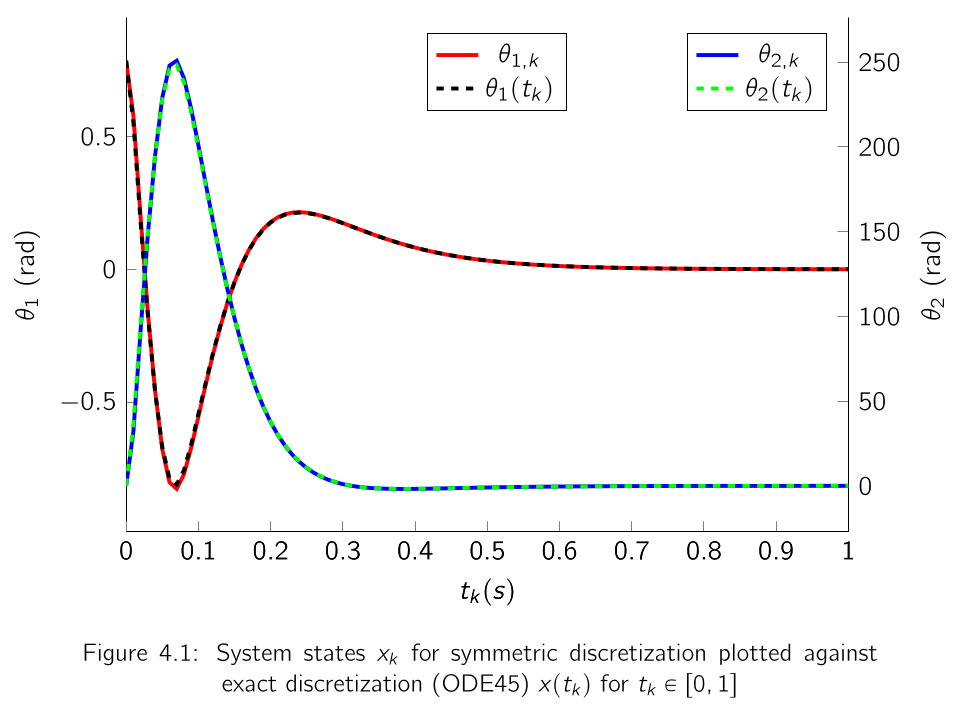
\includegraphics[width=0.8\textwidth]{../Figures/ex1_states.png}
  \end{figure}
\end{frame}

\begin{frame}{Results}
  \begin{figure}[h]
    \centering
    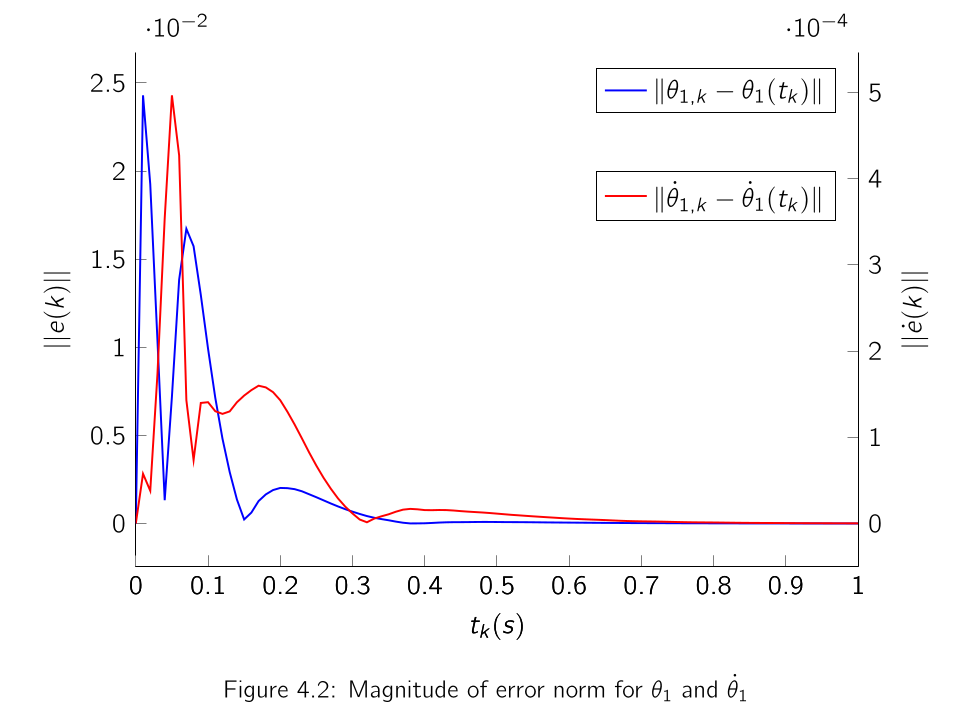
\includegraphics[width=0.8\textwidth]{../Figures/ex1_err1.png}
  \end{figure}
\end{frame}

\begin{frame}{Results}
  \begin{figure}[h]
    \centering
    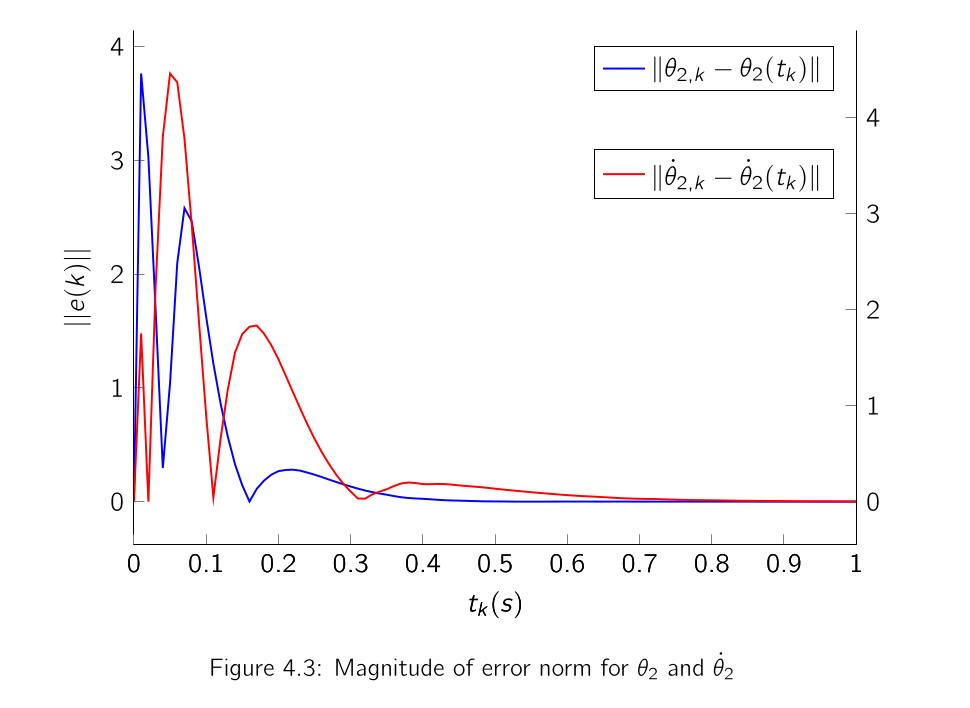
\includegraphics[width=0.8\textwidth]{../Figures/ex1_err2.png}
  \end{figure}
  
\end{frame}

\subsection{TORA System}

\begin{frame}{TORA System}

  \begin{figure}
    \centering
    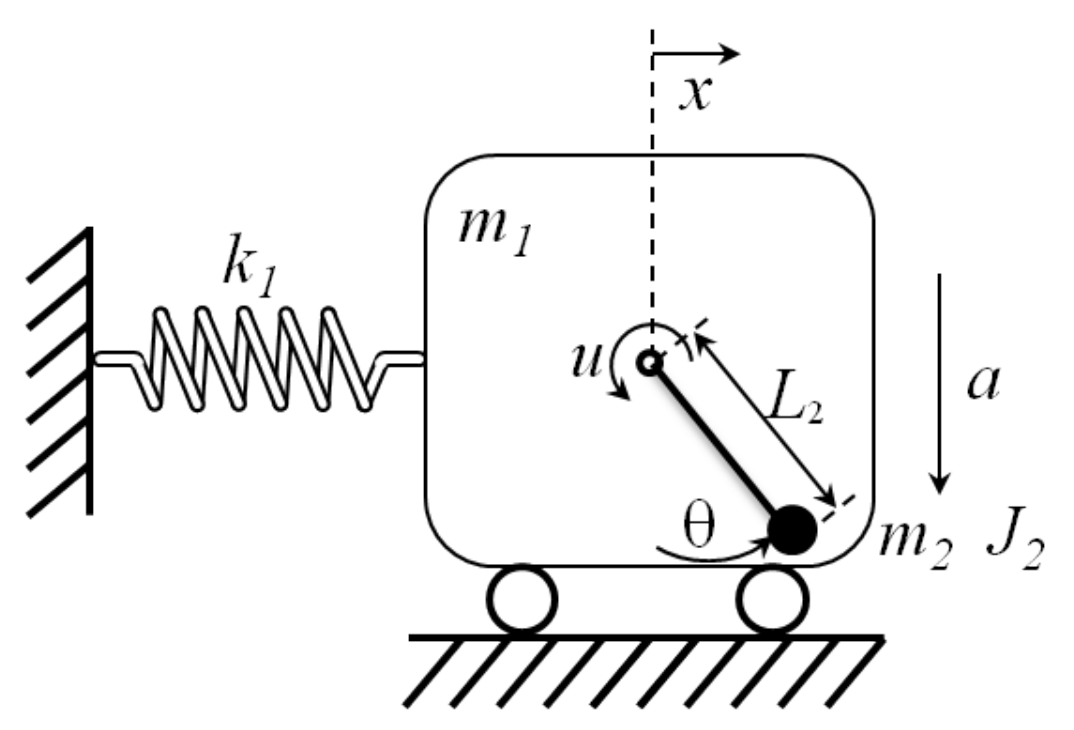
\includegraphics[width=0.6\textwidth]{../Figures/tora.png}
    \caption{Translational Oscillator with Rotational Actuator}
  \end{figure}
  
\end{frame}

\begin{frame}{TORA System - The Dynamical Equations}
  The equations of motion ($M = S^1 \times \R$) are given by:
  \begin{equation}
    \begin{split}
        (m_1 + m_2) \ddot{x} + m_2 L_2 \cos{\theta} \ddot{\theta} - m_2 L_2 \sin{\theta} \dot{\theta}^2 +k_1 x & = 0 \\
        m_2 L_2 \cos{\theta} \ddot{x} + (m_2 L_2^2 + J_2) \ddot{\theta} + m_2L_2 a \sin{\theta} &= u
    \end{split}
  \end{equation}
  
\end{frame}

\begin{frame}{TORA System - General form}
  Taking $(x, \theta) = (x_1, x_2)$ and correspondingly $(\dot{x}, \dot{\theta}) = (y_1, y_2)$, we get the following equations:
  \begin{equation}
  \begin{split}
      \dot{x}_1  & = y_1 \\
      \dot{x}_2  & = y_2 \\
      \dot{y}_1  & = -\Gamma_{22}^1 y_2 y_2 +  e_1 + g_1 u \\
      \dot{y}_2  & = -\Gamma_{22}^2 y^2 y^2 + e_2 + g_2 u
  \end{split}
  \end{equation}

  Here, the Christoffel symbols are non-zero: \vspace{-10pt}

  \begin{equation*}
    \begin{split}
      \Gamma_{22}^1 &= \dfrac{-m_2L_2(m_2L_2^2 + J_2) \sin{x_2}}{(m_1+m_2)(m_2L_2^2 +J_2) - m_2^2L_2^2 \cos^2{x_2}} \\
      \Gamma_{22}^2 &= \dfrac{m_2^2L_2^2 \sin{x_2} \cos{x_2}}{(m_1+m_2)(m_2L_2^2 +J_2) - m_2^2L_2^2 \cos^2{x_2}}
    \end{split}
  \end{equation*}
\end{frame}

\begin{frame}{TORA System - General form}
  \begin{equation*}
      \begin{split}
        e_1 &= \dfrac{m_2^2L_2^2 a \sin{x_2}\cos{x_2} - k_1(m_2L_2^2 + J_2)x_1}{(m_1+m_2)(m_2L_2^2 +J_2) - m_2^2L_2^2 \cos^2{x_2}} \\ 
        e_2 &= \dfrac{-m_2L_2(m_1+m_2)a\sin{x_2} + k_1 m_2L_2 x_1 \cos{x_2}} {(m_1+m_2)(m_2L_2^2 +J_2) - m_2^2L_2^2 \cos^2{x_2}} \\
        g_1 &= \dfrac{-m_2L_2\cos{x_2}}{(m_1+m_2)(m_2L_2^2 +J_2) - m_2^2L_2^2 \cos^2{x_2}} \\
        g_2 &= \dfrac{m_1+m_2}{(m_1+m_2)(m_2L_2^2 +J_2) - m_2^2L_2^2 \cos^2{x_2}}
      \end{split}
  \end{equation*}
\end{frame}

\begin{frame}{TORA System - Feedback Linearization}
  Choosing $\Phi(x,y) = \left( \varphi(x), D\varphi(x)y\right)$, which is given by:

  \begin{equation*}
    \begin{split}
      \tilde{x}_1 &= m_{11}x_1 + m_{12}\sin{x_2}, \
      \tilde{x}_2 = -k_1 x_1 \\
      \tilde{y}_1 &= m_{11}y_1 + m_{12}\cos{x_2}y_2, \
      \tilde{y}_2 = -k_1 y_1
    \end{split}
  \end{equation*}

  Again taking $\tilde{\textbf{x}} = \pmat{\tilde{x}_1 & \tilde{x}_2 & \tilde{y}_1 & \tilde{y}_2 }^T$, such that the linearized equations become $\dfrac{d}{dt} \tilde{\textbf{x}} = A \tilde{\textbf{x}} + B \tilde{u}$
  
\end{frame}

\begin{frame}{TORA System}
  Note that $\tilde{u} = \psi (x, y, u)$ is the auxiliary control, such that:
\begin{equation}
    \tilde{u} = -k_1(-\Gamma_{22}^1 y_2^2 + e_1 + g_1 u)
\end{equation}
Taking $\tilde{u} = -K \tilde{\textbf{x}}$, such that the closed-loop system is stable, we get $\dot{\tilde{\textbf{x}}} = F \tilde{\textbf{x}}$.

We again utilize the symmetric discretization scheme to obtain the discrete-time system.

\end{frame}

\begin{frame}{Results}
  \begin{figure}[h]
    \centering
    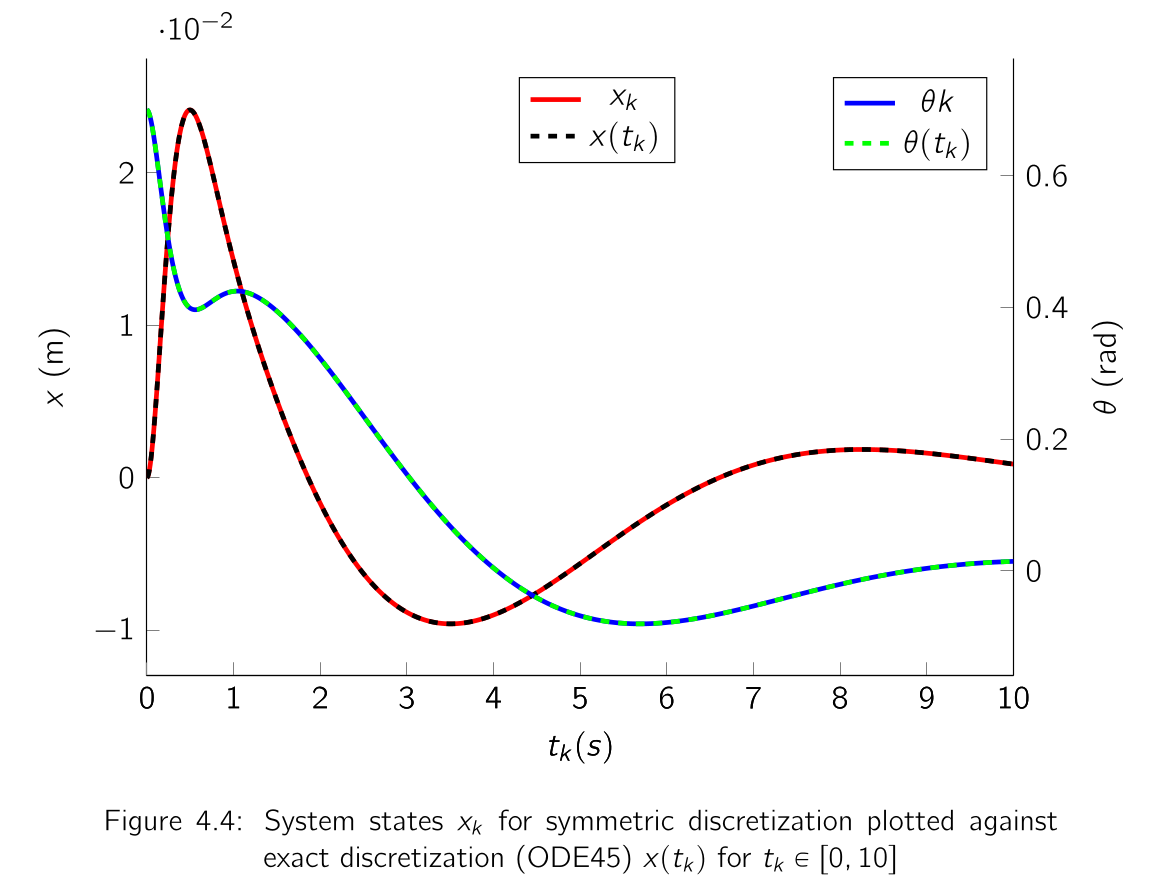
\includegraphics[width=0.8\textwidth]{../Figures/ex2_states.png}
  \end{figure}
\end{frame}

\begin{frame}{Results}
  \begin{figure}[h]
    \centering
    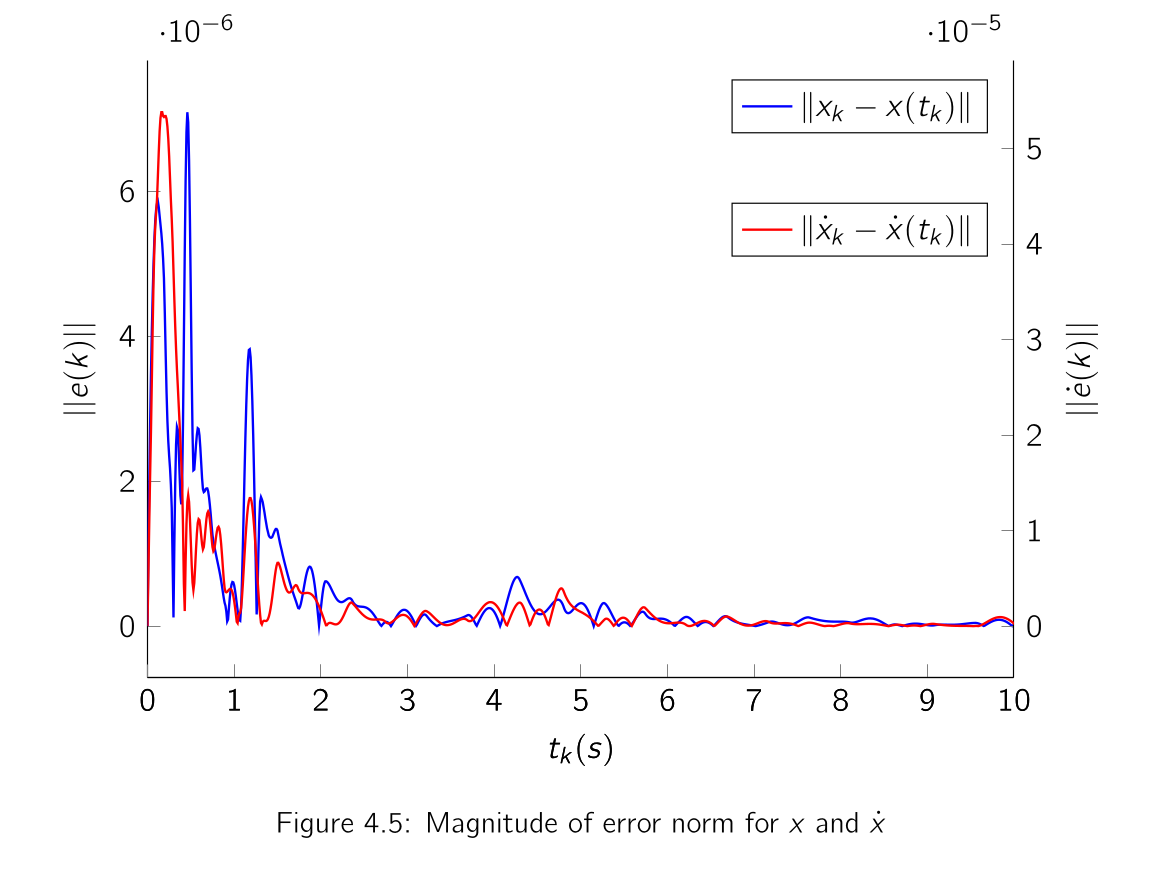
\includegraphics[width=0.8\textwidth]{../Figures/ex2_err1.png}
  \end{figure}
\end{frame}

\begin{frame}{Results}
  \begin{figure}[h]
    \centering
    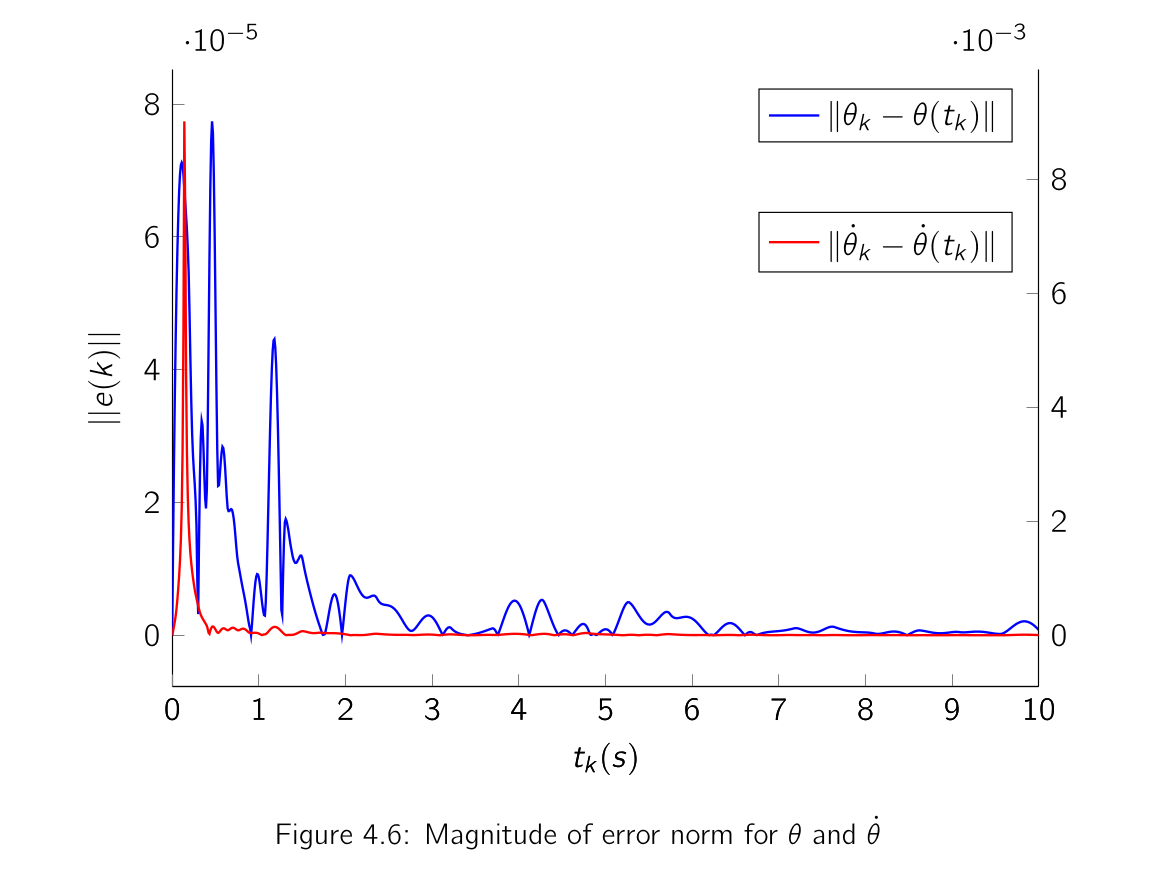
\includegraphics[width=0.8\textwidth]{../Figures/ex2_err2.png}
  \end{figure}
  
\end{frame}

\section*{ }

\begin{frame}{}
  \centering
  \Large \emph{Thank You!}
  
\end{frame}


\end{document}